% A circular diagram of a TeX workflow
% Author: Stefan Kottwitz
% https://www.packtpub.com/hardware-and-creative/latex-cookbook
\documentclass[border=10pt]{standalone}
\usepackage{tikz} 
\usepackage{pgfplots} 

\pgfplotsset{
	axis line style={dashed,opacity=0.4},	
}

\begin{document}
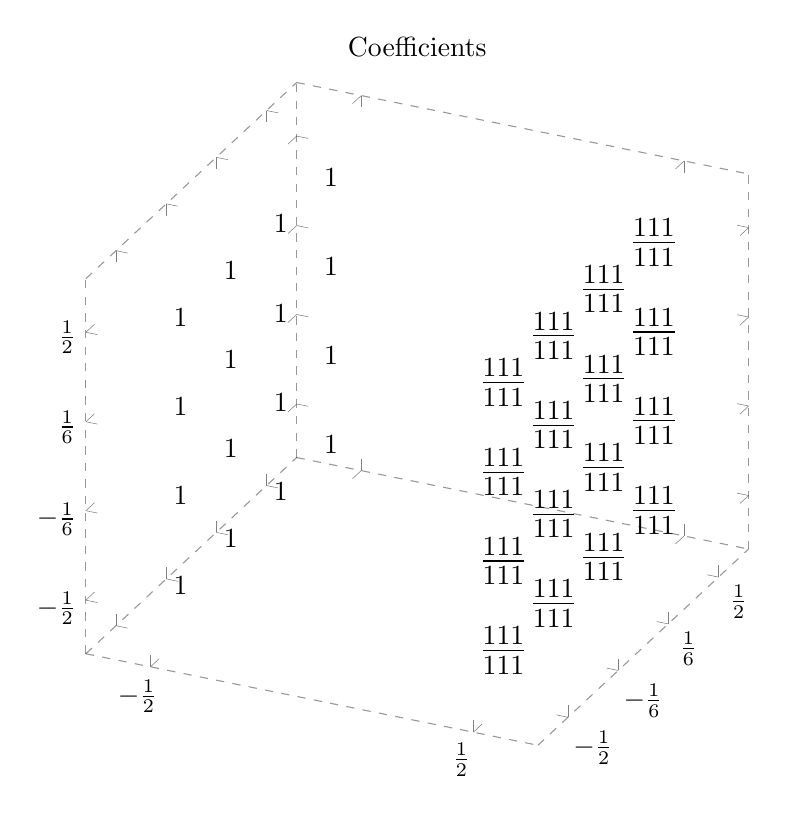
\begin{tikzpicture} 
\begin{axis}
[title=Coefficients,
width = 10cm,
height=10cm,
xmin=-0.7, 
xmax=0.7, 
ymin=-0.7, 
ymax=0.7, 
zmin=-0.7, 
zmax=0.7,
xtick={-0.5,0.5},  
ytick={-0.5,-0.166,0.166,0.5},
ztick={-0.5,-0.166,0.166,0.5},
xticklabels ={$-\frac{1}{2}$,$\frac{1}{2}$},
yticklabels ={$-\frac{1}{2}$,$-\frac{1}{6}$,$\frac{1}{6}$,$\frac{1}{2}$},
zticklabels ={$-\frac{1}{2}$,$-\frac{1}{6}$,$\frac{1}{6}$,$\frac{1}{2}$}]

\node[] at (axis cs:0.5,0.5,0.5) {\Large$\frac{111}{111}$};
\node[] at (axis cs:0.5,0.166,0.5) {\Large$\frac{111}{111}$};
\node[] at (axis cs:0.5,-0.166,0.5) {\Large$\frac{111}{111}$};
\node[] at (axis cs:0.5,-0.5,0.5) {\Large$\frac{111}{111}$};

\node[] at (axis cs:0.5,0.5,0.166) {\Large$\frac{111}{111}$};
\node[] at (axis cs:0.5,0.5,-0.166) {\Large$\frac{111}{111}$};
\node[] at (axis cs:0.5,0.5,-0.5) {\Large$\frac{111}{111}$};

\node[] at (axis cs:0.5,0.166,0.166) {\Large$\frac{111}{111}$};
\node[] at (axis cs:0.5,0.166,-0.166) {\Large$\frac{111}{111}$};
\node[] at (axis cs:0.5,0.166,-0.5) {\Large$\frac{111}{111}$};

\node[] at (axis cs:0.5,-0.166,0.166) {\Large$\frac{111}{111}$};
\node[] at (axis cs:0.5,-0.166,-0.166) {\Large$\frac{111}{111}$};
\node[] at (axis cs:0.5,-0.166,-0.5) {\Large$\frac{111}{111}$};

\node[] at (axis cs:0.5,-0.5,0.166) {\Large$\frac{111}{111}$};
\node[] at (axis cs:0.5,-0.5,-0.166) {\Large$\frac{111}{111}$};
\node[] at (axis cs:0.5,-0.5,-0.5) {\Large$\frac{111}{111}$};


\node[] at (axis cs:-0.5,0.5,0.5) {$1$};
\node[] at (axis cs:-0.5,0.166,0.5) {$1$};
\node[] at (axis cs:-0.5,-0.166,0.5) {$1$};
\node[] at (axis cs:-0.5,-0.5,0.5) {$1$};

\node[] at (axis cs:-0.5,0.5,0.166) {$1$};
\node[] at (axis cs:-0.5,0.5,-0.166) {$1$};
\node[] at (axis cs:-0.5,0.5,-0.5) {$1$};

\node[] at (axis cs:-0.5,0.166,0.166) {$1$};
\node[] at (axis cs:-0.5,0.166,-0.166) {$1$};
\node[] at (axis cs:-0.5,0.166,-0.5) {$1$};

\node[] at (axis cs:-0.5,-0.166,0.166) {$1$};
\node[] at (axis cs:-0.5,-0.166,-0.166) {$1$};
\node[] at (axis cs:-0.5,-0.166,-0.5) {$1$};

\node[] at (axis cs:-0.5,-0.5,0.166) {$1$};
\node[] at (axis cs:-0.5,-0.5,-0.166) {$1$};
\node[] at (axis cs:-0.5,-0.5,-0.5) {$1$};

  \end{axis} 
\end{tikzpicture}
\end{document}

	
	

